\documentclass[crop,tikz]{standalone}

\usepackage[utf8]{inputenc}

% 'crop' is the default for v1.0, before it was 'preview'
%\usetikzlibrary{...}% tikz package already loaded by 'tikz' option

\begin{document}

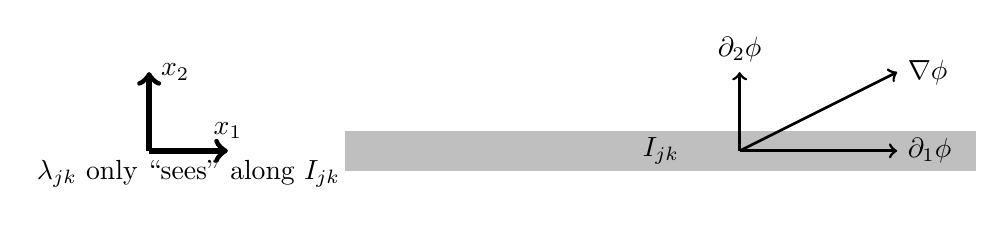
\begin{tikzpicture}
	
	\filldraw[color=black!50!white!50!] (0,0.25) rectangle (8,0.75);
	\node[anchor=center,align=center] at (4,0.5) {$I_{jk}$};
	
	%axes and measure stuff
	\begin{scope}[scale=1.0, shift={(-2.5,0.5)}]
		\draw[->, line width=2pt] (0,0) -- (0,1) node[anchor=west] {$x_2$};
		\draw[->, line width=2pt] (0,0) -- (1,0) node[anchor=south] {$x_1$};
		\node[anchor=north, align=center] at (0.5,0) {$\lambda_{jk}$ only ``sees" along $I_{jk}$};
	\end{scope}
	
	%gradient breakdown into seen and unseen parts
	\begin{scope}[scale=1.0, shift={(5,0.5)}]
		\draw[->, line width=1pt] (0,0) -- (2,1) node[anchor=west] {$\nabla\phi$};
		\draw[->, line width=1pt] (0,0) -- (2,0) node[anchor=west] {$\partial_1\phi$};
		\draw[->, line width=1pt] (0,0) -- (0,1) node[anchor=south] {$\partial_2\phi$};
	\end{scope}
	
\end{tikzpicture}

\end{document}